\documentclass{../../../oss-apphys-exam}
\newcounter{last}

\begin{document}

\gentitle{3}{GAUSS'S LAW, PART 1}

\raggedcolumns

\runningheader{
  \fontfamily{phv}\small
  \textcolor{gray}{AP PHYSICS C: ELECTRICITY AND MAGNETISM $\blacksquare$}
  \textbf{MULTIPLE-CHOICE QUESTIONS}}{}{}


\begin{questions}

  \question A non-conducting sphere does not have a uniform charge density, but
  the density $\rho$ varies with the distance $r$ from the centre of the
  sphere according to the equation $\rho=\beta r$ where $\beta$ is a positive
  constant. The electric field inside the sphere ($r<R$) at a distance $r$
  from the centre of the sphere is
  \begin{choices}
    \choice $\dfrac{\beta r^2}{12\epsilon_0}$
    \choice $\dfrac{\beta r^2}{3\epsilon_0}$
    \choice $\dfrac{\beta r}{2\epsilon_0}$
    \choice $\dfrac{\beta r^2}{2\epsilon_0}$
    \choice $\dfrac{\beta r^2}{4\epsilon_0}$
  \end{choices}
  
  \question What is the electric potential difference between centre and the
  outside surface of the sphere?
  \begin{choices}
    \choice $\dfrac{\beta R^3}{12\epsilon_0}$
    \choice $\dfrac{\beta R}{2\epsilon_0}$
    \choice $\dfrac{\beta R^3}{3\epsilon_0}$
    \choice $\dfrac{\beta R^2}{2\epsilon_0}$
    \choice $\dfrac{\beta R^2}{4\epsilon_0}$
  \end{choices}
    
  \question According to Gauss's law, which of the following statements is
  true?
  \begin{choices}
    \choice It is possible to have a nonzero electric field, but zero electric
    flux.
    \choice It is possible to have a nonzero electric flux, but zero electric
    field.
    \choice It is possible to have a nonzero electric flux through a closed
    surface even if the enclosed charge in a surface is zero.
    \choice If a surface is not closed (such as a sheet of paper), the flux
    through it must be zero.
    \choice It is possible for charges located outside a closed surface to
    produce a net positive flux through the surface.
  \end{choices}
    
  \question According to Gauss's law, the net electric flux passing through a
  closed surface is
  \begin{choices}
    \choice positive if the flux is entering the surface
    \choice negative if the flux is exiting the surface
    \choice positive if the net charge inside the surface is zero
    \choice negative if the net charge inside the surface is zero
    \choice zero if the net charge inside the surface is zero
  \end{choices}
    
    \question Gauss's law is most convenient to use when calculating an electric
    field due to
    \begin{choices}
      \choice charges outside a closed surface
      \choice charges inside a closed surface that has high symmetry
      \choice charges inside a closed surface that has low symmetry
      \choice a potential difference that is negative
      \choice a potential difference that is positive
    \end{choices}
    
  \uplevel{
    \textbf{Question \ref{cube1}-\ref{cube2}}
    \cpic{.27}{cube}
  }
  \question A cube has sides of length $a$. The cube rests so that one side
  rests on the $x$-axis as shown in the figure above. An electric field is
  established in the $x$-direction according to the function $E_x=bx^2$, where
  $b$ is a positive constant. Which of the following statements is true?
  \label{cube1}
  \begin{choices}
    \choice There is a net charge inside the cube.
    \choice There is no net charge inside the cube.
    \choice The flux passing through the cube is negative.
    \choice The flux passing through the cube is zero.
    \choice The flux diminishes while passing through the cube.
  \end{choices}
    
  \question The charge inside the cube can be expressed by the equation
  \label{cube2}
  \begin{choices}
    \choice $\epsilon_0ba$
    \choice $\epsilon_0ba^2$
    \choice $\epsilon_0ba^3$
    \choice $\epsilon_0ba^4$
    \choice $\epsilon_0b^22a^2$
  \end{choices}
   
%    \uplevel{
%      \textbf{Questions \ref{sphere1}--\ref{sphere2}}: A nonconducting spherical
%      charge distribution has a nonuniform positive charge density $\rho$. The
%      centre of the sphere is point $O$, the radius of the sphere is $a$. The
%      sphere is centred on the $x$-axis. A point inside the sphere lies on
%      the $x$-axis at a distance $x_1$ from the centre of the sphere. Another
%      point, $x_2$, is outside the sphere on the $x$-axis.
%      \begin{center}
%        \begin{tikzpicture}
%          \draw[thick] circle(1);
%          \fill circle(.08);
%          \draw[very thick,->] (0,0)--(0,1) node[midway,left]{$a$};
%          \draw[dashed,thick] (0,0)--(6,0) node[right]{\small$\infty$};
%          \fill(.5,0) circle(.05) node[below]{\footnotesize$x_1$};
%          \fill(4,0)  circle(.05) node[below]{\footnotesize$x_2$};
%        \end{tikzpicture}
%      \end{center}
%    }
%
%    \question The electric field at point $x_2$ can be determined by
%    \begin{choices}
%      \choice using Gauss's law to determine the electric field from $O$ to $a$,
%      then using Gauss's law to determine the electric field from $a$ to $x_2$,
%      then finding the difference between the two electric fields.
%      \choice using Gauss's law to determine the electric field from $O$ to $a$,
%      then using Gauss's law to determine the electric field from $a$ to $x_2$,
%      then finding the sum of the two electric fields.
%      \choice integrating the electric potential outside the sphere from
%      infinity to $a$, then integrating the electric potential inside the
%      sphere from $a$ to $x_1$, then finding the difference between the two
%      potential integrals.
%      \choice integrating the electric potential outside the sphere from
%      infinity to $a$, then integrating the electric potential inside the
%      sphere from $a$ to $x_1$, then finding the sum of the two potential
%      integrals.
%      \choice determining the derivative of the potential function inside and
%      outside the sphere, then finding the difference between the two
%      derivatives.
%    \end{choices}
%    \label{sphere1}
%    \vspace{.7in}
%    
%    \question The electric potential at point $x_1$ can be determined by
%    \begin{choices}
%      \choice determining the derivative of the electric field function inside
%      and outside the sphere, then finding the difference between the two
%      derivatives.
%      \choice determining the derivative of the electric field function inside
%      and outside the sphere, then finding the sum of the two derivatives.
%      \choice integrating the derivative of the product of the electric field
%      and potential functions, then finding their sum.
%      \choice integrating the electric field outside the sphere from infinity
%      to $a$, then integrating the electric field inside the sphere from $a$ to
%      $x_1$, then finding the sum of the two potentials.
%      \choice integrating the electric field outside the sphere from infinity
%      to $a$, then integrating the electric field inside the sphere from $a$ to
%      $x_1$, then finding the difference between the two potentials.
%    \end{choices}
%    \label{sphere2}

  \newpage
  
  \uplevel{
    \textbf{Questions \ref{solid1}--\ref{solid2}}: A solid conducting sphere of
    radius $a$ is placed inside a conducting spherical shell of radius $3a$, as
    shown. A charge $+2Q$ is placed on the inner sphere, and a
    charge $-Q$ is placed on the outer sphere.
    \begin{center}
      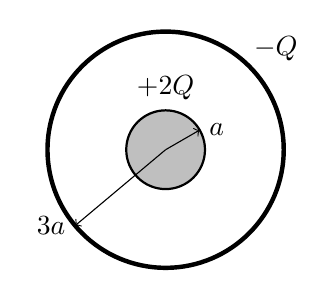
\begin{tikzpicture}[scale=.5]
        \fill circle (.07);
        \draw[thick,fill=lightgray] circle (1);
        \node[thick,above] at (0,1) {$+2Q$};
        \draw[ultra thick] circle (3);
        \node[above right] at (2,2) {$-Q$};
        \draw[rotate=30,->] (0,0)--(1,0) node[right]{$a$};
        \draw[rotate=220,->] (0,0)--(3,0) node[left]{$3a$};
      \end{tikzpicture}
    \end{center}
  }
    
  \question Which of the following graphs best represents the electric field
  $\vec E$ as a function of the distance $r$ from the centre of the spheres?
  
  \begin{oneparchoices}
    \choice
    \begin{tikzpicture}[scale=1.5]
      \draw[axes] (0,0)--(2,0);
      \draw[axes] (0,0)--(0,1.5) node[right]{\small$E$};
      \draw[thick] (.5,.05)--(.5,-.05) node[below]{\small$a$};
      \draw[thick] (1.5,.05)--(1.5,-.05) node[below]{\small$3a$};
      \draw[ultra thick] (0,0) to[out=50,in=260] (.5,1.2)--(1.8,0);
    \end{tikzpicture}
    \choice
    \begin{tikzpicture}[scale=1.5]
      \draw[axes] (0,0)--(2,0);
      \draw[axes] (0,0)--(0,1.5) node[right]{\small$E$};
      \draw[thick] (.5,.05)--(.5,-.05) node[below]{\small$a$};
      \draw[thick] (1.5,.05)--(1.5,-.05) node[below]{\small$3a$};
      \draw[ultra thick] (0,1.2)--(.5,1.2) to[out=-55,in=180] (1.8,.3);
    \end{tikzpicture}
    \choice
    \begin{tikzpicture}[scale=1.5]
      \draw[axes] (0,0)--(2,0);
      \draw[axes] (0,0)--(0,1.5) node[right]{\small$E$};
      \draw[thick] (.5,.05)--(.5,-.05) node[below]{\small$a$};
      \draw[thick] (1.5,.05)--(1.5,-.05) node[below]{\small$3a$};
      \draw[ultra thick] (0,0)--(.5,1.2) to[out=-55,in=180] (1.8,.3);
    \end{tikzpicture}
    \choice
    \begin{tikzpicture}[scale=1.5]
      \draw[axes] (0,0)--(2,0);
      \draw[axes] (0,0)--(0,1.5) node[right]{\small$E$};
      \draw[thick] (.5,.05)--(.5,-.05) node[below]{\small$a$};
      \draw[thick] (1.5,.05)--(1.5,-.05) node[below]{\small$3a$};
      \draw[ultra thick] (0,0)--(.5,0);
      \draw[ultra thick] (0.5,1.2) to[out=-55,in=180] (1.5,.7);
      \draw[ultra thick] (1.5,.5) to[out=-55,in=180] (1.8,.3);
      \fill (.5,1.2) circle (.05);
      \fill (1.5,.5) circle (.05);
    \end{tikzpicture}
    \choice
    \begin{tikzpicture}[scale=1.5]
      \draw[axes] (0,0)--(2,0);
      \draw[axes] (0,0)--(0,1.5) node[right]{\small$E$};
      \draw[thick] (.5,.05)--(.5,-.05) node[below]{\small$a$};
      \draw[thick] (1.5,.05)--(1.5,-.05) node[below]{\small$3a$};
      \draw[ultra thick] (0,0)--(.5,0);
      \draw[ultra thick] (0.5,1.2) to[out=-55,in=180] (1.5,.7);
      \draw[ultra thick] (1.5,0)--(1.8,0);
      \fill (.5,1.2) circle (.05);
      \fill (1.5,.7) circle (.05);
    \end{tikzpicture}
  \end{oneparchoices}
  \label{solid1}
    
  \question Which of the following graphs best represents the electric
  potential $V$ as a function of the distance $r$ from the centre of the
  spheres?
  
  \begin{oneparchoices}
    \choice
    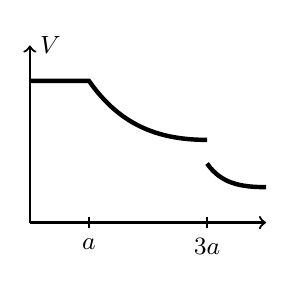
\begin{tikzpicture}[scale=1.5,thick]
      \draw[->] (0,0)--(2,0);
      \draw[->] (0,0)--(0,1.5) node[right]{\small$V$};
      \draw(.5,.05)--(.5,-.05) node[below]{\small$a$};
      \draw(1.5,.05)--(1.5,-.05) node[below]{\small$3a$};
      \draw[ultra thick] (0,1.2)--(.5,1.2) to[out=-55,in=180] (1.5,.7);
      \draw[ultra thick] (1.5,.5) to[out=-55,in=180] (2,.3);
    \end{tikzpicture}
    \choice
    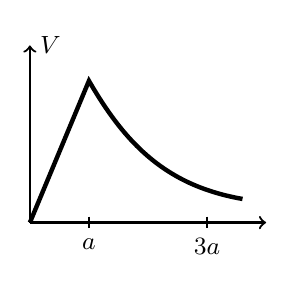
\begin{tikzpicture}[scale=1.5,thick]
      \draw[->] (0,0)--(2,0);
      \draw[->] (0,0)--(0,1.5) node[right]{\small$V$};
      \draw(.5,.05)--(.5,-.05) node[below]{\small$a$};
      \draw(1.5,.05)--(1.5,-.05) node[below]{\small$3a$};
      \draw[ultra thick] (0,0)--(.5,1.2)to[out=-60,in=170] (1.8,.2);
    \end{tikzpicture}
    \choice
    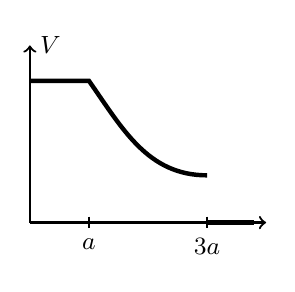
\begin{tikzpicture}[scale=1.5,thick]
      \draw[->] (0,0)--(2,0);
      \draw[->] (0,0)--(0,1.5) node[right]{\small$V$};
      \draw (.5,.05)--(.5,-.05) node[below]{\small$a$};
      \draw (1.5,.05)--(1.5,-.05) node[below]{\small$3a$};
      \draw[ultra thick] (0,1.2)--(.5,1.2) to[out=-55,in=180] (1.5,.4);
      \draw[ultra thick] (1.5,0)--(1.9,0);
    \end{tikzpicture}
    \choice
    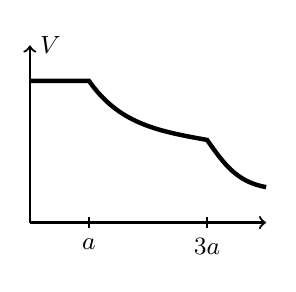
\begin{tikzpicture}[scale=1.5,thick]
      \draw[->] (0,0)--(2,0);
      \draw[->] (0,0)--(0,1.5) node[right]{\small$V$};
      \draw (.5,.05)--(.5,-.05) node[below]{\small$a$};
      \draw (1.5,.05)--(1.5,-.05) node[below]{\small$3a$};
      \draw[ultra thick] (0,1.2)--(.5,1.2)
      to[out=-55,in=170] (1.5,.7) to[out=-55,in=170] (2,.3);
    \end{tikzpicture}
    \choice
    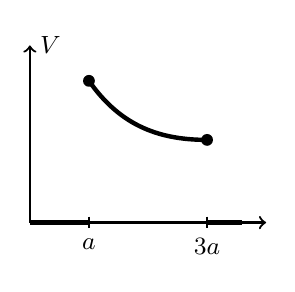
\begin{tikzpicture}[scale=1.5,thick]
      \draw[->] (0,0)--(2,0);
      \draw[->] (0,0)--(0,1.5) node[right]{\small$V$};
      \draw (.5,.05)--(.5,-.05) node[below]{\small$a$};
      \draw (1.5,.05)--(1.5,-.05) node[below]{\small$3a$};
      \draw[ultra thick] (0,0)--(.5,0);
      \draw[ultra thick] (0.5,1.2) to[out=-55,in=180] (1.5,.7);
      \draw[ultra thick] (1.5,0)--(1.8,0);
      \fill (.5,1.2) circle (.05);
      \fill (1.5,.7) circle (.05);
    \end{tikzpicture}   
  \end{oneparchoices}
  \label{solid2}
\end{questions}
\setcounter{last}{\value{question}}
\newpage


\runningheader{
  \fontfamily{phv}\small
  \textcolor{gray}{AP PHYSICS C: ELECTRICITY AND MAGNETISM $\blacksquare$}
  \textbf{FREE-RESPONSE QUESTIONS}}{}{}

% TAKEN FROM 2007 AP PHYSICS C EXAM FREE-RESPONSE QUESTION E&M 2
\begin{center}
  \begin{tikzpicture}[thick,scale=.7]
    \draw[fill=gray!50] circle (3) node[below=45]{\small$-Q$};
    \draw[fill=white] circle (2);
    \draw[fill=gray!50] circle (1) node[below=5]{\small$+Q$};
    
    \fill[rotate=125] (1,0) circle (.075) node[above left=-3]{\small$X$};
    \fill[rotate=120] (2,0) circle (.075) node[below right=-2.5]{\small$Y$};

    \draw[axes,rotate=70] (0,0)--(1,0) node[pos=.7,left=-2]{\small$a$};
    \draw[axes,rotate=25] (0,0)--(2,0) node[pos=.7,above=-1]{\small$2a$};
    \draw[axes,rotate=-25] (0,0)--(3,0) node[pos=.9,above=-1]{\small$3a$};
  \end{tikzpicture}
\end{center}
\begin{questions}
  \setcounter{question}{\value{last}}
  
  \question In the figure above, a nonconducting solid sphere of radius a with
  charge $+Q$ uniformly distributed throughout its volume is concentric with a
  nonconducting spherical shell of inner radius $2a$ and outer radius $3a$ that
  has a charge $-Q$ uniformly distributed throughout its volume. Express all
  answers in terms of the given quantities and fundamental constants.

  \begin{parts}
    \part Using Gauss's law, \textbf{derive} expressions for the magnitude of
    the electric field as a function of radius $r$ in the following regions.
    \begin{subparts}
      \subpart Within the solid sphere ($r<a$)
      \vspace{\stretch1}
      
      \subpart Between the solid sphere and the spherical shell ($a<r<2a$)
      \vspace{\stretch1}
      
      \subpart Within the spherical shell ($2a<r<3a$)
      \vspace{\stretch3}
      \newpage
      
      \subpart Outside the spherical shell ($r>3a$)
      \vspace{\stretch1}
    \end{subparts}
    
    \part What is the electric potential at the outer surface of the spherical
    shell ($r=3a$)? \textbf{Explain} your reasoning.
    \vspace{\stretch2}
    
    \part\textbf{Derive} an expression for the electric potential difference
    $V_X-V_Y$ between points $X$ and $Y$ shown in the figure.
    \vspace{\stretch3}
  \end{parts}
  \newpage

  % TAKEN FROM 2019 AP PHYSICS C E&M EXAM FREE-RESPONSE QUESTION 2. THE QUESTION
  % HAS BEEN SLIGHTLY MODIFIED TO FIT THE FORMATTING STANDARD SINCE 2024
  \uplevel{
    \centering
    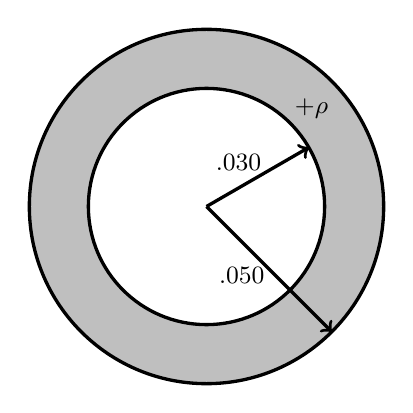
\begin{tikzpicture}[very thick,scale=.75]
      \draw[fill=gray!50] circle (3) node[above right=28]{\small$+\rho$};
      \draw[fill=white] circle (2);
      
      \draw[->,rotate=-45] (0,0)--(3,0)
      node[pos=.55,left]{\small\SI{.050}\metre};

      \draw[->,rotate=30] (0,0)--(2,0)
      node[pos=.75,left=4]{\small\SI{.030}\metre};
    \end{tikzpicture}
  }

  \question A nonconducting hollow sphere of inner radius \SI{.030}{\metre} and
  outer radius \SI{.050}{\metre} carries a positive volume charge density
  $\rho$, as shown in the figure above. The charge density $\rho$ of the sphere
  is given as a function of the distance $r$ from the centre of the sphere, in
  meters, by the following.
  \begin{align*}
    r<\SI{.030}\metre:\quad\quad & \rho = 0\\
    \SI{.030}\metre<r<\SI{.050}\metre:\quad\quad & \rho = \frac br\quad\quad
    \text{where}\quad\quad b = \SI{1.6e-6}{\coulomb\per\metre\squared}\\
    r > \SI{.050}\metre:\quad\quad & \rho = 0
  \end{align*}
  \begin{parts}
    \part\textbf{Calculate} the total charge of the sphere.
    \vspace{\stretch1}
    
    \part Using Gauss's law, \textbf{calculate} the magnitude of the electric
    field $E$ at the outer surface of the sphere.
    \vspace{\stretch1}
    \newpage
    
    \part On the axes below, \textbf{sketch} the magnitude of the electric
    field $E$ as a function of distance $r$ from the centre of the sphere.
    \uplevel{
      \centering
      \begin{tikzpicture}[scale=.9]
        \draw[axes] (0,0)--(10,0) node[right]{$r$ [m]};
        \draw[axes] (0,0)--(0,6) node[above]{$E$};

        \draw[dashed] (4,-.2)--(4,5) node[pos=0,below]{\SI{.030}\metre};
        \draw[dashed] (7,-.2)--(7,5) node[pos=0,below]{\SI{.050}\metre};
      \end{tikzpicture}
    }

    \part\textbf{Calculate} the electric potential $V$ at the outer surface of
    the sphere. Assume the electric potential to be zero at infinity.
    \vspace{\stretch1}
    
    \uplevel{
      A proton is released from rest at the outer surface of the sphere at
      time $t=0$.
    }
    \part\textbf{Calculate} the magnitude of the initial acceleration of the
    proton.
    \vspace{\stretch1}
    
    \part\textbf{Calculate} the speed of the proton after a long time.
    \vspace{\stretch1}
  \end{parts}
  \newpage

  % TAKEN FROM 2012 AP PHYSICS C E&M EXAM FREE-RESPONSE QUESTION 1. THE
  % TIKZ FIGURE BELOW IS A FAIRLY GOOD REPRODUCTION OF THE ORIGINAL AP EXAM
  % DIAGRAM. ALSO, THE FORMATTING OF THE QUESTIONS HAS BEEN MODIFIED TO CONFORM
  % TO THE NEWER STANDARD SINCE 2025
  \uplevel{
    \centering
    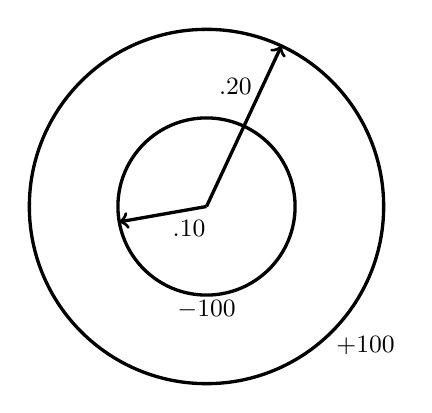
\begin{tikzpicture}[very thick,scale=.75]
      \draw circle (3) node[below right=43]{\small$+\SI{100}\volt$};
      \draw[fill=white] circle (1.5) node[below=30]{\small$\SI{-100}\volt$};

      \draw[->,rotate=190] (0,0)--(1.5,0)
      node[pos=.2,below]{\small\SI{.10}\metre};

      \draw[->,rotate=65] (0,0)--(3,0) node[pos=.75,left]{\small\SI{.20}\metre};
    \end{tikzpicture}
  }
  
  \question Two thin, concentric, conducting spherical shells, insulated from
  each other, have radii of \SI{.10}{\metre} and \SI{.20}{\metre}, as shown
  above. The inner shell is set at an electric potential of \SI{-100}\volt, and
  the outer shell is set at an electric potential of $+\SI{100}\volt$, with each
  potential defined relative to the conventional reference point. Let $Q_i$ and
  $Q_o$ represent the net charge on the inner and outer shells, respectively,
  and let $r$ be the radial distance from the centre of the shells. Express all
  algebraic answers in terms of $Q_i$, $Q_o$, $r$, and fundamental constants,
  as appropriate.
  \begin{parts}
    \part Using Gauss's Law, \textbf{derive} an algebraic expression for the
    electric field $E(r)$ for $\SI{.10}\metre<r<\SI{.20}\metre$.
    \vspace{\stretch1}
    
    \part\textbf{Determine} an algebraic expression for the electric field
    $E(r)$ for   $r>\SI{.20}\metre$.
    \vspace{\stretch1}
    
    \part\textbf{Determine} an algebraic expression for the electric potential
    $V(r)$ for $r>\SI{.20}\metre$.
    \vspace{\stretch1}
    
    \part Using the numerical information given, \textbf{calculate} the value
    of the total charge $Q_T$ on the two spherical shells ($Q_T = Q_i + Q_o$).
    \vspace{\stretch1}
    \newpage
    
    \part On the axes below, \textbf{sketch} the electric field $E$ as a
    function of $r$. Let the positive direction be radially outward.
    \uplevel{
      \centering
      \begin{tikzpicture}
        \draw[axes] (0,0)--(8,0) node[right]{$r$ [m]};
        \draw[axes] (0,-2.5)--(0,2.5) node[above]{$E$};
        \foreach \x in {0.10,0.20,0.30} \draw (\x*20,.1)--+(0,-.2)
        node[below]{$\x$};
      \end{tikzpicture}
    }

    \part On the axes below, \textbf{sketch} the electric potential $V$ as a
    function of $r$.
    \uplevel{
      \centering
      \begin{tikzpicture}
        \draw[axes] (0,0)--(8,0) node[right]{$r$ [m]};
        \draw[axes] (0,-2.5)--(0,2.5) node[above]{$V$};
        \foreach \x in {0.10,0.20,0.30} \draw (\x*20,.1)--+(0,-.2)
        node[below]{$\x$};
      \end{tikzpicture}
  }
  \end{parts}
\end{questions}
\end{document}
